%%==================================================
%% app1.tex for BIT Master Thesis
%% modified by yang yating
%% version: 0.1
%% last update: Dec 25th, 2016

%% modified by Meng Chao
%% version: 0.2
%% last update: May 29th, 2017
%%==================================================


\chapter{单目数据集场景}
\label{DataSets}


\begin{figure}[h]
\centering
	\subfigure[fr2/desk场景]
    {
		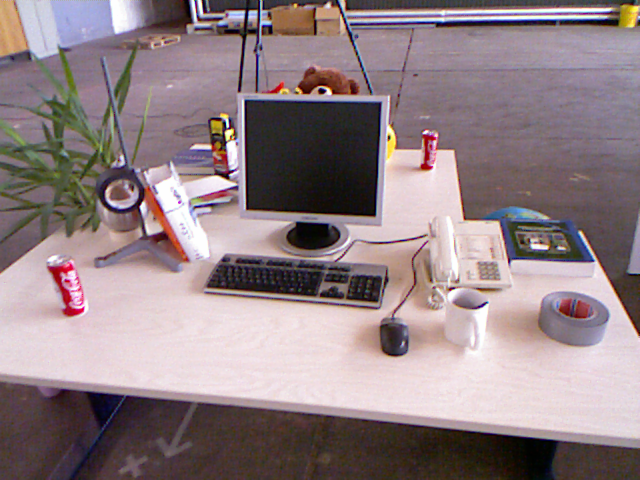
\includegraphics[scale=0.27]{figures/fr2_desk.png}  
	}
	\subfigure[fr3/nostructure\_ texture\_ near\_ with\_ loop场景]
    {	
		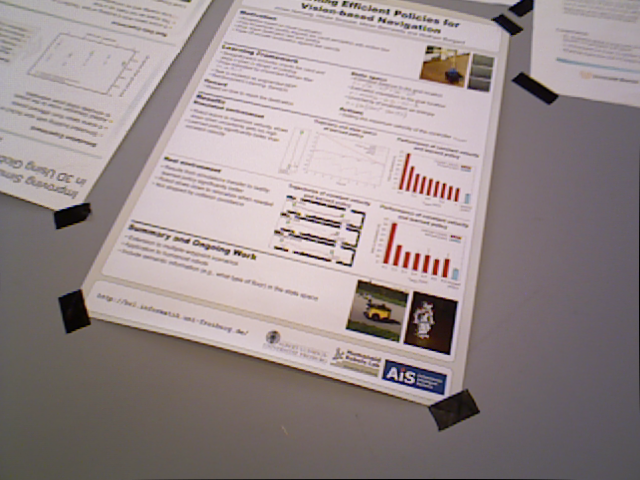
\includegraphics[scale=0.27]{figures/fr3_nostructure.png}
	}
	\subfigure[fr3/long\_ office\_ household场景]
    {	
		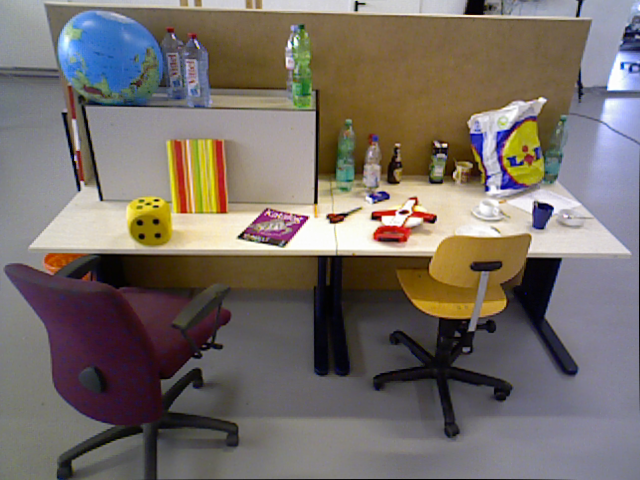
\includegraphics[scale=0.27]{figures/fr3_long_office.png}
	}
\caption{TUM RGBD数据集}
\end{figure}


\begin{figure}[h]
\centering
	\subfigure[MH场景]
    {
		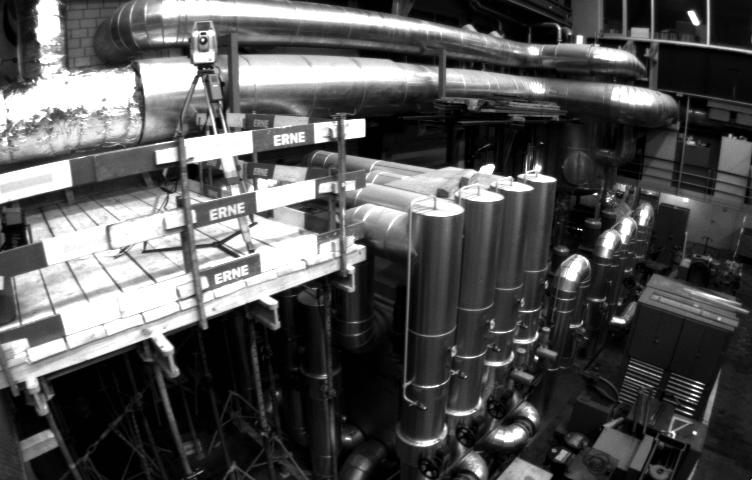
\includegraphics[scale=0.25]{figures/MH.png}  
	}
	\subfigure[V1场景]
    {	
		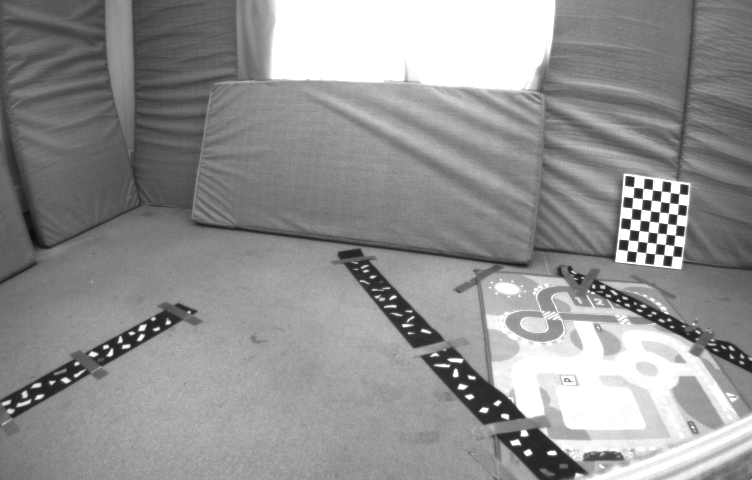
\includegraphics[scale=0.25]{figures/V1.png}
	}
\caption{EuRoC数据集}
\end{figure}





